% ─────────────────────────────────────────────────────────────────────────────
% Sec. 5  Experiments. Tables / figures are generated by results/paper/build_paper_results.py
% (re-run it after new results arrive; cells still missing print as a red "?").
% Needs in preamble.tex: \usepackage{multirow} \usepackage{colortbl} \definecolor{oursbg}{HTML}{E8F0FC}
% ─────────────────────────────────────────────────────────────────────────────
\section{Experiments}
\label{sec:exp}

Our central claim is that the memory and latency of \method do not grow with the input resolution,
while its accuracy matches the strongest token-pruning methods. \cref{sec:main} compares accuracy under
memory and token budgets, \cref{sec:scaling} varies the resolution, and \cref{sec:ablation} studies the
components of \method.

\providecommand{\pend}{\textcolor{red}{?}}

\begin{table*}[t]
  \centering
  \footnotesize
  \setlength{\tabcolsep}{4pt}
  \begin{tabular}{l cc c cc c ccc}
    \toprule
    & \multicolumn{2}{c}{Document} & Real-world & \multicolumn{2}{c}{High resolution} & & \multicolumn{3}{c}{Saving \vs uncompressed$\uparrow$} \\
    \cmidrule(lr){2-3}\cmidrule(lr){4-4}\cmidrule(lr){5-6}\cmidrule(lr){8-10}
    Method & DocVQA & InfoVQA & MME-RW & HR-Bench 4K & V$^*$ Bench & Avg.\ (\%) & TTFT & Memory & FLOPs \\
    \midrule
    \multicolumn{10}{c}{\textit{Upper bound: all visual tokens}} \\
    Uncompressed & 91.4 & 78.7 & 51.6 & 62.0 & 83.8 & 100.0 & 1.0$\times$ & 1.0$\times$ & 1.0$\times$ \\
    \midrule
    \multicolumn{10}{c}{\textit{Budget $B=1536$ visual tokens (default), $\approx$21\% of all visual tokens}} \\
    FastV~\cite{fastv} & 84.0 & 61.0 & 46.9 & \underline{59.0} & 79.1 & 90.0 & 2.5$\times$ & 1.5$\times$ & 2.9$\times$ \\
    SparseVLM~\cite{sparsevlm} & 55.1 & 62.2 & \underline{50.2} & \textbf{59.5} & \underline{79.6} & 85.5 & 2.2$\times$ & 1.5$\times$ & 2.4$\times$ \\
    VisionZip~\cite{visionzip} & 48.7 & 47.6 & 41.7 & 49.0 & 70.2 & 71.5 & \underline{2.7$\times$} & \underline{4.2$\times$} & \underline{3.2$\times$} \\
    HiRED~\cite{hired} & 58.5 & 51.6 & 45.2 & 53.5 & 72.8 & 78.0 & \textbf{2.8$\times$} & 3.7$\times$ & \textbf{3.3$\times$} \\
    IF-Prune~\cite{ifprune} & \textbf{88.2} & \underline{72.7} & 49.3 & 57.5 & \textbf{81.7} & \underline{94.9} & 1.5$\times$ & 0.7$\times$ & 1.8$\times$ \\
    \rowcolor{oursbg}
    \method (ours) & \underline{87.0}$^{\downarrow}$ & \textbf{74.8}$^{\uparrow}$ & \textbf{52.1}$^{\uparrow}$ & 56.5 & 77.5 & \textbf{95.0} & 2.4$\times$ & \textbf{5.0$\times$} & \underline{3.2$\times$} \\
    \midrule
    \multicolumn{10}{c}{\textit{Budget $B=2560$ visual tokens, $\approx$35\% of all visual tokens}} \\
    FastV~\cite{fastv} & \underline{89.6} & 70.5 & 50.1 & \underline{59.0} & \underline{81.7} & 95.5 & 2.0$\times$ & 1.5$\times$ & 2.2$\times$ \\
    SparseVLM~\cite{sparsevlm} & 69.8 & 71.1 & \underline{51.8} & 57.0 & 81.2 & 91.2 & 1.7$\times$ & 1.4$\times$ & 1.8$\times$ \\
    VisionZip~\cite{visionzip} & 62.8 & 57.9 & 45.9 & 57.5 & 76.4 & 83.0 & \underline{2.1$\times$} & \underline{2.8$\times$} & \underline{2.4$\times$} \\
    HiRED~\cite{hired} & 67.8 & 59.2 & 48.2 & 58.0 & 77.5 & 85.8 & \textbf{2.2$\times$} & 2.6$\times$ & \textbf{2.5$\times$} \\
    IF-Prune~\cite{ifprune} & \underline{89.6} & \underline{74.8} & 49.9 & \textbf{59.5} & \textbf{83.8} & \underline{97.1} & 1.3$\times$ & 0.7$\times$ & 1.5$\times$ \\
    \rowcolor{oursbg}
    \method (ours) & \textbf{90.1} & \textbf{78.6}$^{\uparrow}$ & \textbf{52.2} & 58.0 & 79.6 & \textbf{97.6} & 1.7$\times$ & \textbf{3.6$\times$} & 2.2$\times$ \\
    \midrule
    \multicolumn{10}{c}{\textit{Budget $B=3072$ visual tokens, $\approx$42\% of all visual tokens}} \\
    FastV~\cite{fastv} & \textbf{90.8} & 73.6 & 49.7 & \textbf{61.0} & \underline{82.7} & 97.2 & \underline{1.8$\times$} & 1.5$\times$ & \underline{2.0$\times$} \\
    SparseVLM~\cite{sparsevlm} & 69.8 & 72.5 & \underline{51.0} & 57.0 & \textbf{83.8} & 91.8 & 1.5$\times$ & 1.3$\times$ & 1.6$\times$ \\
    VisionZip~\cite{visionzip} & 68.8 & 61.8 & 47.4 & 56.5 & 78.5 & 86.1 & \textbf{1.9$\times$} & \underline{2.4$\times$} & \textbf{2.2$\times$} \\
    HiRED~\cite{hired} & 71.1 & 61.8 & 49.2 & \underline{60.0} & 81.7 & 89.2 & \textbf{1.9$\times$} & 2.3$\times$ & \textbf{2.2$\times$} \\
    IF-Prune~\cite{ifprune} & 90.1 & \underline{75.1} & 49.8 & \textbf{61.0} & 82.2 & \underline{97.4} & 1.2$\times$ & 0.7$\times$ & 1.4$\times$ \\
    \rowcolor{oursbg}
    \method (ours) & \underline{90.3} & \textbf{79.4}$^{\uparrow}$ & \textbf{53.5}$^{\uparrow}$ & 59.5 & 81.7 & \textbf{99.3} & 1.4$\times$ & \textbf{2.7$\times$} & 1.8$\times$ \\
    \bottomrule
  \end{tabular}
  \caption{\textbf{Accuracy and cost on InternVL3.5-8B.} Scores on each benchmark; Avg.\ is the mean percentage of the uncompressed score over the five benchmarks. HR-Bench 8K is in \cref{tab:hr8k}. Cost is the saving relative to the uncompressed model (higher is better), averaged over the five benchmarks. $^{\uparrow}$/$^{\downarrow}$: \method is significantly better/worse than the strongest baseline on that benchmark (paired bootstrap, 95\%); unmarked differences are not significant. Best compressed result per budget in \textbf{bold}, second \underline{underlined}.}
  \label{tab:main}
\end{table*}


% ─────────────────────────────────────────────────────────────────────────────
\subsection{Setup}
\label{sec:setup}

\paragraph{Models and benchmarks.}
We evaluate on InternVL3.5-4B, -8B, and -14B~\cite{internvl35}, and use the 8B model unless stated
otherwise. We cover three kinds of high-resolution inputs: documents (DocVQA val~\cite{docvqa}, 5,349
questions; InfoVQA val~\cite{infovqa}, 2,801), real-world scenes (MME-RealWorld Lite~\cite{mmerealworld},
1,919), and very high-resolution images with small targets (HR-Bench 4K and 8K~\cite{hrbench}, 800
questions each; V$^*$ Bench~\cite{vstar}, 191). We report ANLS on DocVQA and InfoVQA, CircularEval
accuracy on HR-Bench (a question counts only if all four option orders are answered correctly), and
multiple-choice accuracy otherwise. All methods use greedy decoding and the same prompts, and start
from the same official dynamic tiling with up to $N_{\max}=47$ tiles plus a thumbnail. Averages in
\cref{tab:main} are over the first five benchmarks; HR-Bench 8K is used for the resolution study of
\cref{sec:scaling}.

\paragraph{Baselines.}
We compare with FastV~\cite{fastv}, SparseVLM~\cite{sparsevlm}, VisionZip~\cite{visionzip}, and
IF-Prune~\cite{ifprune}, ported to InternVL3.5 from the official code with the official
hyperparameters: FastV and IF-Prune prune at layer 2, IF-Prune uses the released InternVL2.5-1B guide
model, SparseVLM prunes at the official relative depths with its pruning rate calibrated per budget,
and VisionZip keeps dominant and contextual tokens in each tile. For all methods, the budget $B$ is the
number of visual tokens left in the KV cache. We also compare with two same-budget downscaling baselines
(\cref{sec:downscale}). Implementation details are in the supplementary material.

\paragraph{Efficiency measurement.}
All measurements use one NVIDIA A6000 (48\,GB), bfloat16, and batch size 1. TTFT is the wall-clock time
to the first generated token, including the vision encoder and any scoring or guide model, and we report the median over 50 images per benchmark after one warm-up image. Memory is the peak
allocated GPU memory minus the model weights; for IF-Prune it includes the guide model. FLOPs count the
vision encoder and the prefill up to the first token.

\paragraph{Protocol.}
All \method hyperparameters are fixed on held-out calibration data (\cref{sec:impl}), except for the attention layers, which were chosen in preliminary experiments and are disclosed in the supplementary material; no test set is used for any other choice. We test differences with a paired bootstrap over questions (or CircularEval groups) at
95\% confidence.

% ─────────────────────────────────────────────────────────────────────────────
\subsection{Accuracy under a memory budget}
\label{sec:main}

\providecommand{\pend}{\textcolor{red}{?}}

\begin{table}[t]
  \centering
  \footnotesize
  \setlength{\tabcolsep}{2.2pt}
  \begin{tabular}{l cccc}
    \toprule
    & \multicolumn{4}{c}{Memory limit per image} \\
    \cmidrule(lr){2-5}
    Method & $\leq$0.5\,GB & $\leq$1\,GB & $\leq$2\,GB$^\dagger$ & None \\
    \midrule
    FastV & -- & -- & \underline{97.2}\,{\tiny (3072)} & 97.2\,{\tiny (3072)} \\
    SparseVLM & -- & -- & 91.8\,{\tiny (3072)} & 91.8\,{\tiny (3072)} \\
    VisionZip & 71.5\,{\tiny (1536)} & 86.1\,{\tiny (3072)} & 86.1\,{\tiny (3072)} & 86.1\,{\tiny (3072)} \\
    HiRED & \underline{72.3}\,{\tiny (1024)} & \underline{89.2}\,{\tiny (3072)} & 89.2\,{\tiny (3072)} & 89.2\,{\tiny (3072)} \\
    IF-Prune & -- & -- & -- & \underline{97.4}\,{\tiny (3072)} \\
    \rowcolor{oursbg}
    \method (ours) & \textbf{95.0}\,{\tiny (1536)} & \textbf{99.3}\,{\tiny (3072)} & \textbf{99.3}\,{\tiny (3072)} & \textbf{99.3}\,{\tiny (3072)} \\
    \bottomrule
  \end{tabular}
  \caption{\textbf{Accuracy under a memory limit} on InternVL3.5-8B: the best mean percentage of the uncompressed score (five benchmarks of \cref{tab:main}) that each method reaches with budgets $B\in\{1024,\dots,3072\}$ while its peak memory on top of the model weights stays within the limit (budget in parentheses; --: no budget fits; $^\dagger$the memory of the uncompressed model). FastV, SparseVLM, and IF-Prune need at least 1.3\,GB at any budget, and IF-Prune needs more memory than the uncompressed model.}
  \label{tab:memcap}
\end{table}


The number of high-resolution requests a GPU can serve is bounded by memory, so we first ask which
accuracy each method reaches within a memory limit (\cref{tab:memcap}). \method is the most accurate
method under every limit. Within 1\,GB per image, it retains 99.3\% of the uncompressed accuracy, while
FastV, SparseVLM, and IF-Prune cannot run at any budget, and VisionZip reaches 86.1\%. IF-Prune even needs
more memory than the uncompressed model (3.0 \vs 2.0\,GB), mainly for its guide model, so it does not fit
within the uncompressed model's own footprint. Without a limit, \method still has the highest accuracy
(99.3\% at $B=3072$).

\cref{tab:main} compares all methods at equal token budgets. At the default budget $B=1536$, which keeps
about a fifth of the visual tokens, \method retains 95.0\% of the uncompressed accuracy on average, the
highest of all methods, ahead of IF-Prune (94.9\%), FastV (90.0\%), SparseVLM (85.5\%), and VisionZip
(71.5\%). It needs 5.0$\times$ less memory than the uncompressed model, against 1.5$\times$ for FastV and SparseVLM and
0.7$\times$ for IF-Prune, and it is 1.6$\times$ faster than IF-Prune. From $B=1536$ upward,
\method has the highest average accuracy of all methods at every budget, reaching 99.3\% at $B=3072$,
while using the least memory.

\method is strongest where the answer depends on the layout of the whole image. On InfoVQA it is
significantly better than every baseline at every budget, by 2.1 to 4.3 points over the strongest one,
and on MME-RealWorld it even exceeds the uncompressed model (significantly at $B=3072$, +1.9 points):
its high-resolution scenes contain large regions irrelevant to the question, and keeping only the
coverage view and the question-relevant tiles removes these distractors, which may also explain why more
tiles lower the accuracy of the uncompressed model on HR-Bench 8K (\cref{tab:hr8k}). On HR-Bench and V$^*$ Bench, which ask about
small objects, \method is within a few points of the best baseline, and none of these differences is
significant at any budget.

\begin{figure}[t]
  \centering
  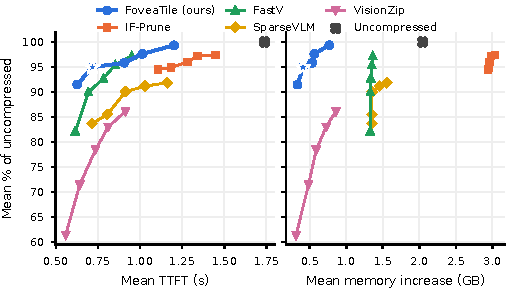
\includegraphics[width=\linewidth]{figures/fig_pareto.pdf}
  \caption{\textbf{Accuracy--cost trade-off} on InternVL3.5-8B, averaged over the five benchmarks of \cref{tab:main}, for
  $B\in\{1024,1536,2048,2560,3072\}$. The star marks the default \method budget. \method uses the least
  memory at every budget, and every configuration of IF-Prune and SparseVLM is dominated by a \method
  configuration that is both faster and more accurate.}
  \label{fig:pareto}
\end{figure}

\cref{fig:pareto} shows the full trade-off over five budgets. In memory, \method has the best curve at every budget: even its largest budget uses less memory than any budget of FastV, SparseVLM,
or IF-Prune. In TTFT, \method reaches the highest accuracy of all methods (99.3\% at 1.2\,s), and every
configuration of IF-Prune and SparseVLM is dominated by a \method configuration that is both faster and
more accurate: at about the same TTFT as IF-Prune at $B=1536$ (1.2\,s), \method reaches 99.3\% instead
of 94.9\%, and at $B=1536$ (95.0\%) it is more accurate than IF-Prune at any $B\leq1536$ with about
0.6$\times$ its TTFT and one seventh of its memory.

\begin{table}[t]
  \centering
  \footnotesize
  \setlength{\tabcolsep}{3.4pt}
  \begin{tabular}{l cc cc cc}
    \toprule
    & \multicolumn{2}{c}{$B=1536$} & \multicolumn{2}{c}{$B=2560$} & \multicolumn{2}{c}{$B=3072$} \\
    \cmidrule(lr){2-3}\cmidrule(lr){4-5}\cmidrule(lr){6-7}
    Method & Avg. & Small & Avg. & Small & Avg. & Small \\
    \midrule
    Low-Res & 84.2 & 73.5 & 92.9 & 85.4 & 93.3 & 85.9 \\
    Low-Res-Fill & 91.7 & 82.6 & 94.1 & 86.6 & 96.2 & 90.3 \\
    \rowcolor{oursbg}
    \method (ours) & \textbf{95.0} & \textbf{91.9} & \textbf{97.6} & \textbf{93.8} & \textbf{99.3} & \textbf{95.5} \\
    \bottomrule
  \end{tabular}
  \caption{\textbf{Same-budget downscaling}, as a percentage of the uncompressed score. Avg.: the five benchmarks of \cref{tab:main}; Small: HR-Bench 4K, HR-Bench 8K, and V$^*$. Low-Res is the official tiling capped at $K=B/256$ tiles, which cannot always fill the budget (on average 1{,}149/1{,}931/1{,}972 visual tokens); Low-Res-Fill gives the whole budget to coverage tiles ($m{=}K$). Per-benchmark scores and paired confidence intervals are in the supplementary material.}
  \label{tab:downscale}
\end{table}


\paragraph{Same-budget downscaling.}
\label{sec:downscale}
A simpler way to meet the budget is to downscale the image. We test two versions at the same $B$: the
official tiling capped at $K=B/256$ tiles (Low-Res), and the coverage tiles of \method given the whole
budget ($m{=}K$, Low-Res-Fill). \method retains more of the uncompressed accuracy at every budget
(95.0/97.6/99.3\% \vs 91.7/94.1/96.2\% for Low-Res-Fill, \cref{tab:downscale}), and the gap is largest on
the small-object benchmarks (91.9/93.8/95.5\% \vs 82.6/86.6/90.3\%). On HR-Bench and V$^*$ Bench, \method is
ahead of Low-Res-Fill in all nine comparisons, by 2.5 to 8.0 points, significantly on HR-Bench 8K at
$B=1536$; on MME-RealWorld it is significantly better at every budget. Spending part of the budget on
question-relevant detail tiles is thus better than spending all of it on a uniformly sharper view.

\paragraph{Model scale.}
With the hyperparameters calibrated on the 8B model, \method reaches 94.5\% and 95.2\% on InternVL3.5-4B
and \mbox{-14B} at $B=1536$, with peak memory of 0.37 and 0.43\,GB, about 7$\times$ less than IF-Prune. The full
table is in the supplementary material.

% ─────────────────────────────────────────────────────────────────────────────
\subsection{Memory and latency that do not grow with resolution}
\label{sec:scaling}

\begin{figure}[t]
  \centering
  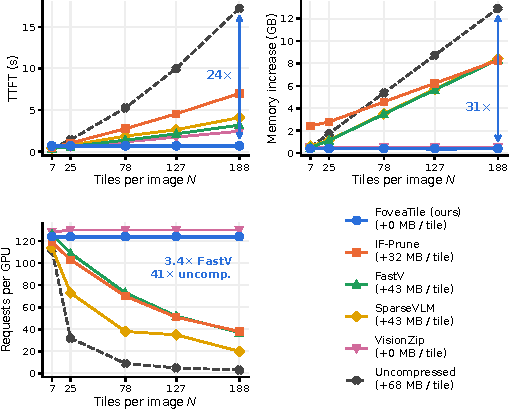
\includegraphics[width=\linewidth]{figures/fig_scaling.pdf}
  \caption{\textbf{Cost as the input resolution grows} (HR-Bench 8K, $B=1536$; the tile cap is raised so
  that the same images split into 7 to 188 tiles). The legend gives the growth of peak memory per added
  tile. \method stays flat in TTFT, memory, and requests per GPU, while every method that prunes inside
  the language model degrades with $N$.}
  \label{fig:scaling}
\end{figure}

\providecommand{\pend}{\textcolor{red}{?}}

\begin{table}[t]
  \centering
  \footnotesize
  \setlength{\tabcolsep}{3.2pt}
  \begin{tabular}{l ccc ccc}
    \toprule
    & \multicolumn{3}{c}{25 tiles} & \multicolumn{3}{c}{188 tiles} \\
    \cmidrule(lr){2-4}\cmidrule(lr){5-7}
    Method & Acc. & TTFT & Mem. & Acc. & TTFT & Mem. \\
    \midrule
    Uncompressed & 56.5 & 1.44 & 1.79 & 49.0 & 17.22 & 12.90 \\
    \midrule
    FastV & \textbf{54.0} & 0.63 & 1.16 & 42.5 & 3.19 & 8.34 \\
    SparseVLM & 53.5 & 0.76 & 1.18 & 51.5 & 4.09 & 8.44 \\
    VisionZip & 44.5 & \textbf{0.58} & 0.49 & 27.0 & 2.45 & 0.49 \\
    HiRED & 48.5 & \textbf{0.58} & 0.54 & 41.0 & 2.35 & 0.88 \\
    IF-Prune & 52.5 & 1.04 & 2.81 & \textbf{52.0} & 7.00 & 8.28 \\
    \rowcolor{oursbg}
    \method (ours) & 52.0 & 0.70 & \textbf{0.42} & 47.0 & \textbf{0.71} & \textbf{0.41} \\
    \bottomrule
  \end{tabular}
  \caption{\textbf{Higher input resolution at a fixed budget} ($B=1536$) on HR-Bench 8K. Raising the tile cap from $N_{\max}=47$ to 200 splits each image into 188 tiles instead of about 25. Acc.\ is CircularEval accuracy, TTFT in seconds, Mem.\ in GB.}
  \label{tab:hr8k}
\end{table}


To isolate the effect of resolution, we raise the tile cap on HR-Bench 8K so that the same images are
split into 7 to 188 tiles, and measure cost at $B=1536$ (\cref{fig:scaling}). The peak memory of \method
does not grow at all: it stays at 0.41\,GB from 7 to 188 tiles, because no stage of \method ever holds
more than the budget. Every method that prunes inside the language model grows linearly with $N$, by
32 to 43\,MB per added tile (68\,MB for the uncompressed model), and needs over 8\,GB at 188 tiles,
20$\times$ more than \method. TTFT behaves the same way: \method stays at 0.7\,s, whereas FastV and
IF-Prune become 4.5$\times$ and 10$\times$ slower than \method at 188 tiles, and the uncompressed model
24$\times$ slower. VisionZip also keeps its memory flat, since it prunes before the language model, but
it still encodes every tile, so its TTFT grows with $N$, and its accuracy is 23.5 points lower on average
(\cref{tab:main}). \method is the only method whose memory and latency are both independent of the
resolution. Beyond about 35 tiles, \method is the fastest of all methods, and its lead grows with
$N$.

Memory determines how many requests a GPU can serve. We measure this directly: on one A6000 (33\,GB free
after the 8B weights), we prefill requests one after another, keep the KV cache of each, as if it were
still decoding, and count the requests that complete before the GPU runs out of memory. \method holds 124
requests at every resolution, from 7 to 188 tiles. With FastV and IF-Prune this number falls from 103--109
at 25 tiles to 37--38 at 188 tiles, with SparseVLM to 20, and with the uncompressed model from 32 to 3. At
188 tiles, \method serves 3.4$\times$ more requests than FastV, 3.3$\times$ more than IF-Prune,
6.2$\times$ more than SparseVLM, and 41$\times$ more than the uncompressed model.

\cref{tab:hr8k} reports accuracy at both resolutions. Splitting the image more finely at a fixed budget
lowers accuracy for every method, and even for the uncompressed model (56.5 to 49.0). Among the
compressed methods, \method has the best accuracy per unit cost: at 188 tiles it is 10$\times$ faster
than IF-Prune and 6$\times$ faster than SparseVLM with 20$\times$ less memory, and it is more accurate
than FastV (47.0 \vs 42.5) at 4.5$\times$ less TTFT. With a larger budget
($B=2560$), \method matches the best compressed methods at 188 tiles (52.5) and exceeds the uncompressed
model (49.0), which may suffer from the very long visual sequence.

% ─────────────────────────────────────────────────────────────────────────────
\subsection{Ablations}
\label{sec:ablation}

\providecommand{\pend}{\textcolor{red}{?}}

\begin{table}[t]
  \centering
  \footnotesize
  \setlength{\tabcolsep}{2.6pt}
  \begin{tabular}{l ccc cc c}
    \toprule
    Variant & Info & MME & Local & Avg. & Worst & TTFT \\
    \midrule
    \rowcolor{oursbg}
    \method & 94.4 & 97.1 & 100.1 & 95.8 & 85.4 & 0.92 \\
    Coverage only, $m{=}K$ & 95.8 & 95.6 & 95.8 & 95.7 & 77.5 & 0.58 \\
    Thumbnail, $m{=}1$ & 86.6 & 90.8 & 95.6 & 88.7 & 75.7 & -- \\
    Prior only, $S{=}0$ & 94.5 & 93.6 & 92.6 & 94.1 & 78.5 & 0.73 \\
    Window $2\times$ & 94.2 & 97.6 & 98.4 & 95.9 & 85.0 & 1.11 \\
    Window $4\times$ & 94.5 & 96.6 & 97.0 & 95.5 & 80.9 & 1.48 \\
    Random prior & 85.9 & 87.7 & 90.2 & 86.8 & 70.6 & -- \\
    \bottomrule
  \end{tabular}
  \caption{\textbf{Ablations} on the held-out calibration sets of \cref{sec:impl} (Info, MME), as a percentage of the uncompressed score. Local: MME-RealWorld remote sensing, monitoring, and autonomous driving. Worst: lowest percentage among InfoVQA and the five MME-RealWorld subtasks. Window sizes are relative to the default $S$; TTFT in seconds.}
  \label{tab:ablation}
\end{table}


\cref{tab:ablation} ablates the components of \method on the held-out calibration sets, averaged over
five budgets. Using the thumbnail alone as coverage ($m=1$) loses 7.1 points on average, so giving
the coverage tiles half of the budget is essential. Using only coverage tiles ($m=K$) gives the same average
as \method at lower TTFT, but its worst task drops from 85.4\% to 77.5\% and the local-detail subtasks
from 100.1\% to 95.8\%: detail tiles do not raise the average, they prevent failures on questions about
small regions. On the test sets, the same variant trails \method by 3.1 to 3.5 points in average retention
(Low-Res-Fill in \cref{tab:downscale}). Removing boundary scoring ($S=0$) costs 1.7 points on average, 6.9 on the worst task, and
7.5 on local-detail questions, so ranking by the prior alone is not enough. Larger windows add TTFT
without improving accuracy. Finally, replacing the question-aware prior with a random ranking, while
keeping boundary scoring, costs 9.0 points on average and 14.8 on the worst task: which detail tiles reach
the window matters most, and the attention of the VLM over the coverage tiles is what finds them. These accuracy results complement the
recall analysis of \cref{sec:reliability}.
